% ---
% Capa
% ---
\imprimircapa
% ---

% ---
% Folha de rosto
% (o * indica que haverá a ficha bibliográfica)
% ---
\imprimirfolhaderosto*
% ---

% ---
% Inserir a ficha bibliografica
% ---
% http://ficha.bu.ufsc.br/
\begin{fichacatalografica}
	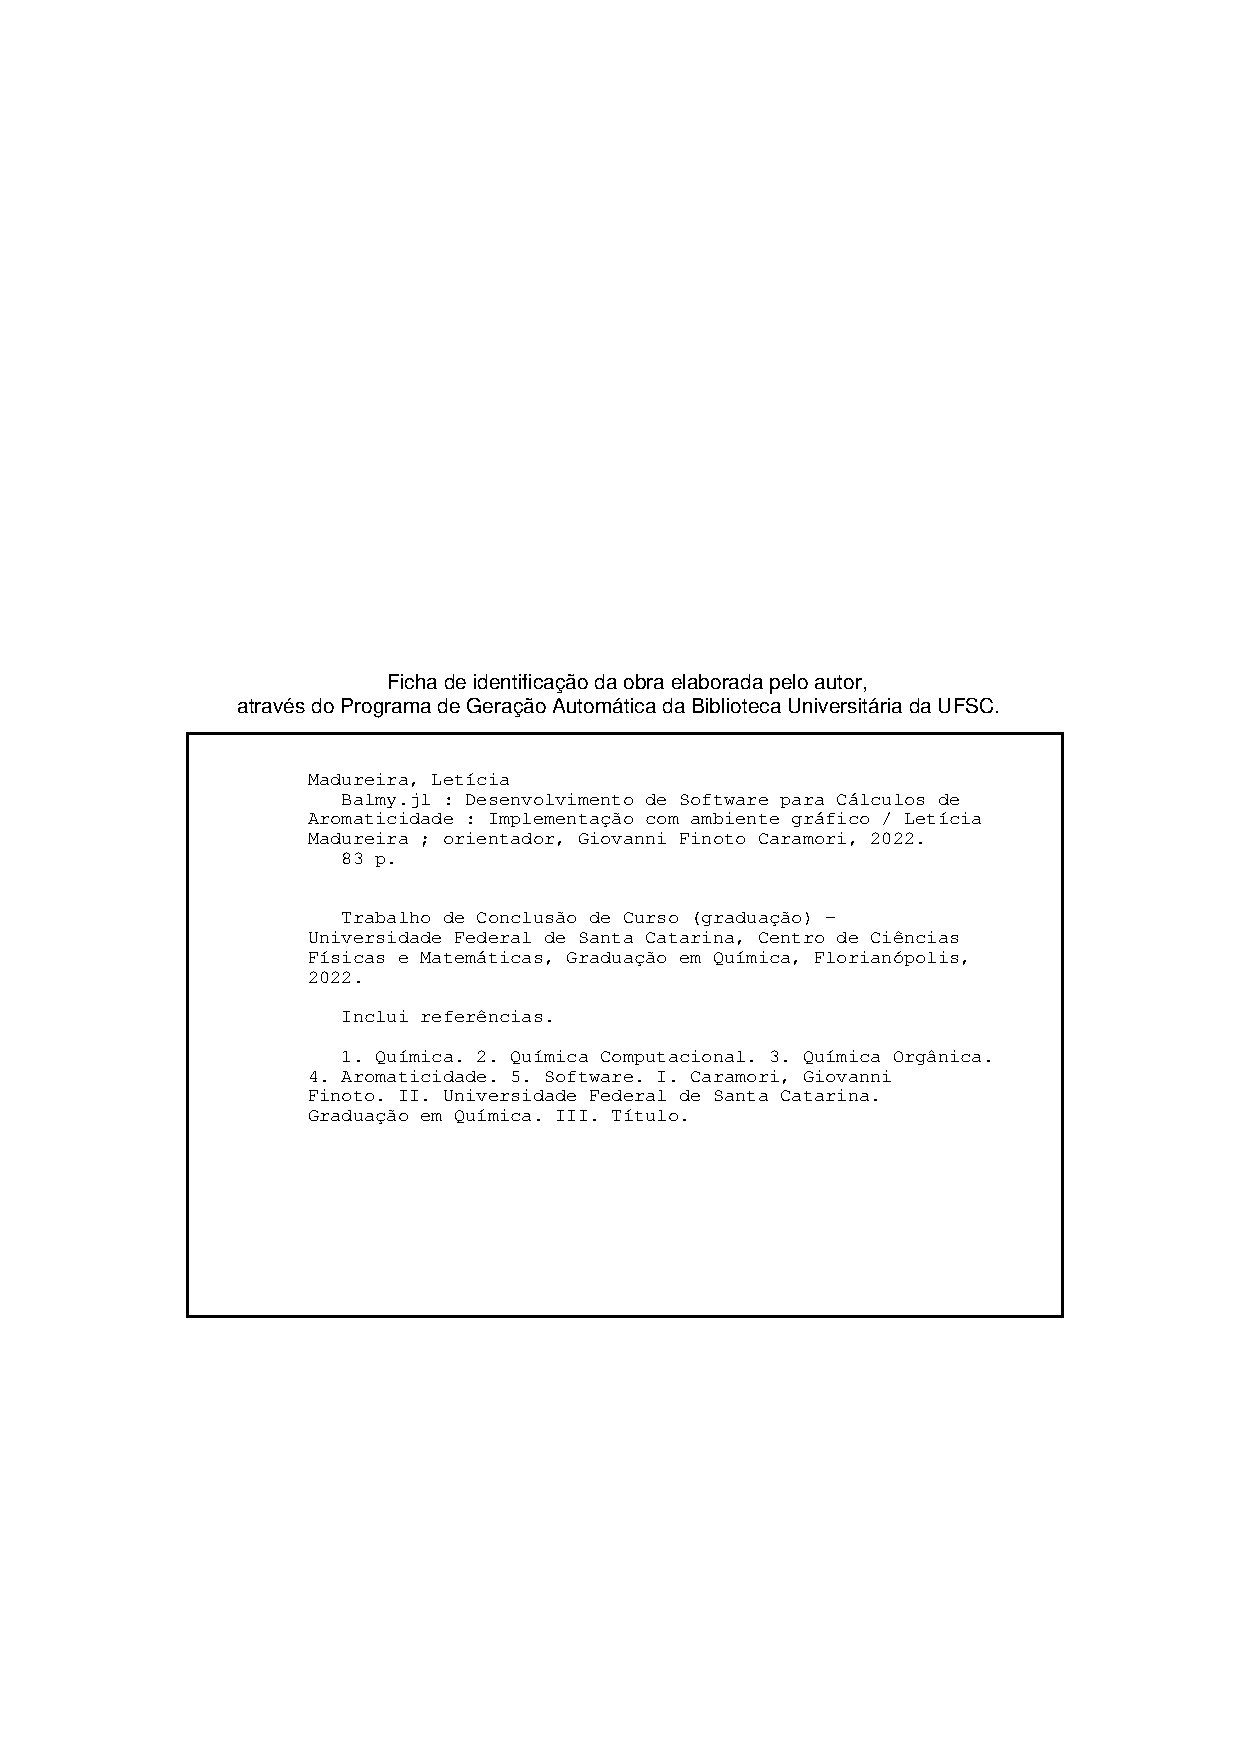
\includepdf{beforetext/Ficha_Catalografica.pdf}
\end{fichacatalografica}
% ---

% ---
% Inserir folha de aprovação
% ---
\begin{folhadeaprovacao}
	\OnehalfSpacing
	\centering
	\imprimirautor\\%
	\vspace*{10pt}		
	\textbf{\imprimirtitulo}%
	\ifnotempty{\imprimirsubtitulo}{:~\imprimirsubtitulo}\\%
	%		\vspace*{31.5pt}%3\baselineskip
	\vspace*{\baselineskip}
	%\begin{minipage}{\textwidth}
	% ~do~\imprimirprograma~do~\imprimircentro~da~\imprimirinstituicao~para~a~obtenção~do~título~de~\imprimirformacao.
	Este~\imprimirtipotrabalho~foi julgado adequado para obtenção do Título de ~\imprimirformacao~e aprovado em sua forma final pelo~\imprimirprograma. \\
		\vspace*{\baselineskip}
	\imprimirlocal, \imprimirdata. \\
	\vspace*{2\baselineskip}
	\assinatura{\OnehalfSpacing\imprimircoordenador \\ \imprimircoordenadorRotulo~do Curso}
	\vspace*{2\baselineskip}
	\textbf{Banca Examinadora:} \\
	\vspace*{\baselineskip}
	\assinatura{\OnehalfSpacing\imprimirorientador \\ \imprimirorientadorRotulo}
	%\end{minipage}%
	\vspace*{\baselineskip}
	\assinatura{Prof.(a) xxxx, Dr(a).\\
	Avaliador(a) \\
	Instituição xxxx}

	\vspace*{\baselineskip}
	\assinatura{Prof.(a) xxxx, Dr(a).\\
	Avaliador(a) \\
	Instituição xxxx}


\end{folhadeaprovacao}
% ---

% ---
% Dedicatória
% ---
\begin{dedicatoria}
	\vspace*{\fill}
	\noindent
	\begin{adjustwidth*}{}{5.5cm}     
		Este trabalho aos meus pais, meu orientador, e aos meus colegas de laboratório.
	\end{adjustwidth*}
\end{dedicatoria}
% ---

% ---
% Agradecimentos
% ---
\begin{agradecimentos}
	Gostaria de tecer um agradecimento primeiro à Universidade Federal de Santa Catarina e ao ensino público de qualidade (e que assim permaneça!), aos meus pais, por sempre terem me dado todo o suporte necessário para o aprendizado independentemente de qualquer entrave, e à minha irmã, por sempre ter me animado nos períodos difíceis, e aos meus 8 gatos, principalmente o Chokito, por ser o companheiro de estudos mais fiel que alguém poderia ter.

Não poderia deixar de citar todos os professores do Departamento de Química, particularmente o meu orientador Giovanni F. Caramori, que me ouviu, me ensinou e se tornou um exemplo de cientista para mim, por sua seriedade, compaixão e amor ao conhecimento. 

Seria injusto não agradecer meus colegas de laboratório, especialmente o Matheus Colaço, pelo carinho e confiança, o Felipe Schneider, pelas conversas e dicas valiosas para a construção deste projeto, e o Denner, pela amizade e descontração.

Como menção honrosa, cito a Alexandra Elbakyan, pois sem a criação do SciHub, a bibliografia do referido documento estaria vazia. Além disso, coloco aqui meu respeito a todas às mulheres na ciência e tecnologia que construíram (e que ainda hão de construir) um caminho que me possibilita estar aqui e desenvolver este trabalho. É uma grande honra fazer parte dessa história.
\end{agradecimentos}
% ---

% ---
% Epígrafe
% ---
\begin{epigrafe}
	\vspace*{\fill}
	\begin{flushright}
		\textit{``
		Classification and theory are not ends in themselves. If they generate new experimental work, new compounds, new processes, new methods - they are good;
		if they are sterile - they are bad  \\
		(Bergmann, E. D, 1971)}
	\end{flushright}
\end{epigrafe}
% ---

% ---
% RESUMOS
% ---

% resumo em português
\setlength{\absparsep}{18pt} % ajusta o espaçamento dos parágrafos do resumo
\begin{resumo}
	\SingleSpacing
    Na química, é comum deparar-se com análises qualitativas de fenômenos através do uso de conceitos multidimensionais bastante difundidos, como a aromaticidade, por exemplo, descrita através de critérios geométricos, magnéticos e topológicos. De maneira geral e sucinta, é estabelecido que um composto aromático apresenta uma estabilização (entenda-se, decréscimo de energia e, consequentemente, de reatividade) devido à deslocalização eletrônica. Isso pode ser analisado de formas diversas, seja calculando a alternância dos comprimentos de ligação e/ou comparando as energias dos orbitais moleculares de fronteira de um composto aromático com um análogo sem deslocalização eletrônica. Nesse sentido, o presente trabalho mostra a ferramenta computacional produzida (chamada \textit{Balmy.jl}) com as linguagens de programação \gls{CSS}, \gls{HTML}, JavaScript e Julia para representar moléculas e seus orbitais tridimensionalmente, utilizando somente o navegador de \textit{internet} para realizar cálculos de índices \gls{HOMA}, \gls{HOMED} e \gls{EHMO}. Os resultados apresentados demostram que os valores de \textit{gap} entre o \gls{HOMO} e o \gls{LUMO} estão de acordo com aqueles apresentados pela literatura. Os resultados coerentes para as energias eletrônicas provam que a aplicação \textit{web} produzida é funcional e está bem implementada, podendo ser usada para análises rápidas da aromaticidade e como ferramenta didática de ensino.
	
	\textbf{Palavras-chave}: Aromaticidade. Multidimensional. \textit{Balmy.jl}. \gls{HOMA}. \gls{HOMED}. \gls{EHMO}
\end{resumo}

% resumo em inglês
\begin{resumo}[Abstract]
	\SingleSpacing
	\begin{otherlanguage*}{english}
In chemistry, it is common to encounter qualitative analyses of phenomena through the use of multidimensional concepts, such as aromaticity, for example, which is defined through the geometric, magnetic, and topological effects observed in molecules. Succinctly, it is established that an aromatic compound presents a stabilization (that is, a decrease in energy and, consequently, in reactivity) due to electron delocalization. This can be analyzed in various ways, either by calculating the alternation of bond lengths and/or comparing the energies of the molecular orbitals at the boundary of an aromatic compound with an analog without electron delocalization. In this sense, the present work shows the tool produced (called Balmy.jl) using the \gls{CSS}, \gls{HTML}, JavaScript, and Julia to represent molecules and their orbitals three-dimensionally, using only the web browser to \gls{HOMA}, and \gls{EHMO}. The results show good agreement with the values of \gls{HOMO}-\gls{LUMO} gaps presented in the literature. The electronic energies consistent results prove that the web application is functional and well implemented, and can be used for aromaticity analysis and as a didactic teaching tool.
		
		\textbf{Keywords}: Aromaticity. Multidimensional. Balmy.jl. \gls{HOMA}. \gls{HOMED}. \gls{EHMO}.
	\end{otherlanguage*}
\end{resumo}

%% resumo em francês 
%\begin{resumo}[Résumé]
% \begin{otherlanguage*}{french}
%    Il s'agit d'un résumé en français.
% 
%   \textbf{Mots-clés}: latex. abntex. publication de textes.
% \end{otherlanguage*}
%\end{resumo}
%
%% resumo em espanhol
%\begin{resumo}[Resumen]
% \begin{otherlanguage*}{spanish}
%   Este es el resumen en español.
%  
%   \textbf{Palabras clave}: latex. abntex. publicación de textos.
% \end{otherlanguage*}
%\end{resumo}
%% ---

{%hidelinks
	\hypersetup{hidelinks}
	% ---
	% inserir lista de ilustrações
	% ---
	\pdfbookmark[0]{\listfigurename}{lof}
	\listoffigures*
	\cleardoublepage
	% ---
	
	% ---
	% inserir lista de quadros
	% ---
	%%\pdfbookmark[0]{\listofquadrosname}{loq}
	%%\listofquadros*
	%%\cleardoublepage
	% ---
	
	% ---
	% inserir lista de tabelas
	% ---
	\pdfbookmark[0]{\listtablename}{lot}
	\listoftables*
	\cleardoublepage
	% ---
	
	% ---
	% inserir lista de abreviaturas e siglas (devem ser declarados no preambulo)
	% ---
	\imprimirlistadesiglas
	% ---
	
	% ---
	% inserir lista de símbolos (devem ser declarados no preambulo)
	% ---
	% \imprimirlistadesimbolos
	% ---
	
	% ---
	% inserir o sumario
	% ---
	\pdfbookmark[0]{\contentsname}{toc}
	\tableofcontents*
	\cleardoublepage
	
}%hidelinks
% ---